\item \textbf{{[}JJC/PRELIM/9597/2018/P1/Q3{]} }

The class \texttt{Node} has the following properties and methods: 
\begin{center}
\begin{tabular}{|l|l|}
\hline 
\multicolumn{2}{|c|}{\texttt{Class: Node}}\tabularnewline
\hline 
\multicolumn{2}{|c|}{Attributes}\tabularnewline
\hline 
\texttt{\textbf{\hspace{0.01\columnwidth}}}\textbf{Identifier} & \texttt{\textbf{\hspace{0.05\columnwidth}}}\textbf{Description}\tabularnewline
\hline 
\texttt{data : String} & Data stored at the node.\tabularnewline
\hline 
\texttt{left : INTEGER} & Points to the left child of the node. Implement 0 as NULL value. \tabularnewline
\hline 
\texttt{right : INTEGER } & Points to the right child of the node. Implement 0 as NULL value.\tabularnewline
\hline 
\multicolumn{2}{|l|}{Methods}\tabularnewline
\hline 
\texttt{Constructor()} & Initialises an instance of \texttt{Node}. \tabularnewline
\hline 
\texttt{set\_data(data : String)} & Modifier method for \texttt{data}.\tabularnewline
\hline 
\texttt{get\_data() : String} & Accessor method for \texttt{data}. \tabularnewline
\hline 
\texttt{set\_left(index : INTEGER)} & Modifier method for \texttt{left}.\tabularnewline
\hline 
\texttt{get\_left() : INTEGER} & Accessor method for \texttt{left}\tabularnewline
\hline 
\texttt{set\_right(index : INTEGER)} & Modifier method for \texttt{right}.\tabularnewline
\hline 
\texttt{get\_right() : INTEGER} & Accessor method for \texttt{right}.\tabularnewline
\hline 
\end{tabular}
\par\end{center}

\subsection*{Task 3.1 }

Write program code for the class \texttt{Node}. 

\subsection*{Evidence 11:}

Program code for Task 3.1.\hfill{} {[}4{]}

The class \texttt{BinarySearchTree} has the following properties and
methods: 
\begin{itemize}
\item Properties 
\begin{itemize}
\item \texttt{root : INTEGER} Points to the root of binary search tree.
Implement 0 as NULL value. 
\item \texttt{nodes : ARRAY{[}31{]} OF Node} The array index starts at 1
and the dataset (i.e.: binary search tree) has a maximum of 31 Node
objects. 
\item \texttt{nextFree : INTEGER} Index for the next unused node. 
\end{itemize}
\item Methods 
\begin{itemize}
\item \texttt{Constructor()} Initialises the \texttt{root}, \texttt{nextFree}
and nodes of \texttt{BinarySearchTree}. 
\item \texttt{addNode(data : String)} Inserts new node into binary search
tree. 

The \texttt{data} of each parent node is larger than the \texttt{data}
of its left child. 
\item \texttt{set\_root(index : INTEGER)} Modifier method for root. 
\item \texttt{get\_root() : INTEGER} Accessor method for root. 
\item \texttt{searchNode(item : String) : BOOLEAN} Searches if \texttt{item}
is stored in one of the nodes of the binary search tree. 

Returns \texttt{TRUE} if found and \texttt{FALSE} otherwise. 
\item \texttt{inOrderTraversal(root : INTEGER)} Displays the \texttt{data}
of each \texttt{node} stored in the binary search tree when traversed
using an inorder algorithm. 

For example: 
\begin{center}
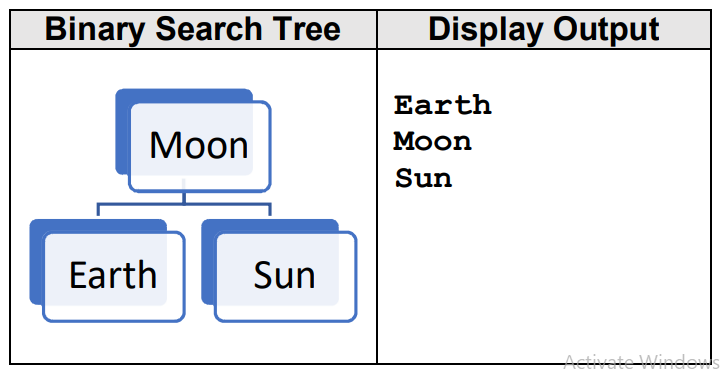
\includegraphics[width=0.5\paperwidth]{C:/Users/Admin/Desktop/Github/question_bank/LyX/static/img/9597-JJC-2018-P1-Q3-1}
\par\end{center}
\item \texttt{balance() : BinarySearchTree} Traverses the binary search
tree to return a new balanced binary search tree. A \textbf{recursive}
algorithm is required. 
\end{itemize}
\end{itemize}

\subsection*{Task 3.2 }

Write program code for the class \texttt{BinarySearchTree}. You may
assume space will not be reused should any node be deleted and the
binary search tree will not be full. 

\subsection*{Evidence 12: }

Program code for Task 3.2. \hfill{}{[}18{]}

The class \texttt{HashTable} has the following properties and methods:

\subsection*{Task 3.3}

Write program code for the class HashTable.
\begin{itemize}
\item properties
\begin{itemize}
\item \texttt{size : INTEGER} Number of items in the hash table array.
\item \texttt{hashTableArray : ARRAY{[}size{]} OF BinarySearchTree} An array
storing \texttt{BinarySearchTree} objects from indices 0 to size -1. 
\end{itemize}
\item methods
\begin{itemize}
\item \texttt{Constructor(size : INTEGER)} Initialises the \texttt{size}
and \texttt{hashTableArray} of \texttt{HashTable}. 
\item \texttt{hash(key : String) : INTEGER} A hashing function that calculates
the address of the hash table. 

Takes \texttt{key}, a String, as an argument. The last six characters
in \texttt{key} are digits.

\textbf{Sums each of the first three digits}, divides the total by
\texttt{size} and returns the remainder. 

For example, where \texttt{size} is 5: 

\noindent\begin{minipage}[t]{1\columnwidth}%
\texttt{hash(\textquotedblleft 111JalanTenteram}\texttt{\textbf{322111}}\texttt{\textquotedblright )}

\texttt{>\textcompwordmark >\textcompwordmark > 2 }

\texttt{hash(\textquotedblleft 23PasirRisAve}\texttt{\textbf{4520021}}\texttt{\textquotedblright )}

\texttt{>\textcompwordmark >\textcompwordmark > 2 }%
\end{minipage}
\end{itemize}
\end{itemize}

\subsection*{Evidence 13: }

Program code for Task 3.3.\hfill{} {[}4{]}

ACE OF CODERS PTE LTD would like to conduct a lucky draw. Each customer
is entitled to submit one entry. All customer data entered is stored
in the text file \texttt{CUSTOMERDATA.txt}. The format of the text
file is as follows: 
\noindent \begin{center}
\texttt{<CUSTOMER NAME> <CONTACT NUMBER>|<ADDRESS> }
\par\end{center}

Below is a sample of \texttt{CUSTOMERDATA.txt}: 

\noindent\fbox{\begin{minipage}[t]{1\columnwidth - 2\fboxsep - 2\fboxrule}%
\texttt{Felicia Lee Si Ying 98635610}\texttt{\textbf{|}}\texttt{19JalanTenteram322019 }

\texttt{Yap Chee How 67767515}\texttt{\textbf{|}}\texttt{23TohTuckDrive608023 }

\texttt{Christy Lopez 92233123}\texttt{\textbf{|}}\texttt{507WestCoastRoad120507 }%
\end{minipage}}

There will be five lucky draw winners. The company has identified
five regions in Singapore and would like to pick one winner from each
region. The hashing function from Task 3.3 \uline{will categorise
an address in one of the five regions}. 

\subsection*{Task 3.4 }

Using the classes programmed previously, code a main program that
repeatedly: 
\begin{itemize}
\item displays the following menu:

\noindent\fbox{\begin{minipage}[t]{1\columnwidth - 2\fboxsep - 2\fboxrule}%
\texttt{1. Prepare hash table}

\texttt{2. Generate winners}

\texttt{3. Search for entry }%
\end{minipage}}
\item calls an appropriate procedure depending on the user\textquoteright s
choice
\end{itemize}
When implementing the choices, take note of the following: 
\begin{enumerate}
\item[1.] \textbf{ Prepare hash table} 

User inputs suitable size of hash table to be initialised.

Reads customer data from \texttt{CUSTOMERDATA.txt}. 

Uses address as key and customer name, contact number as value.

Stores the customer names, contact numbers into the hash table. 
\item[2.] \textbf{ Generate winners} 

Randomly select one winner from each binary search tree in the hash
table.

Display their names and contact numbers. 
\item[3.]  \textbf{Search for entry} 

Staff of the company may not enter the lucky draw. 

Displays whether the staff name and contact number entered by user
exists in the hash table. 
\end{enumerate}

\subsection*{Evidence 14: }

Program code for Task 3.4. \hfill{}{[}10{]}

\subsection*{Task 3.5}

Run your program. Complete choice 1 before searching the following. 

\noindent\begin{minipage}[t]{1\columnwidth}%
\texttt{>\textcompwordmark >\textcompwordmark > Sandra Chelvan 92233123 }

\texttt{>\textcompwordmark >\textcompwordmark > Haz Awang 87767888 }

\texttt{>\textcompwordmark >\textcompwordmark > Seah Hon Hui 91144000 }%
\end{minipage}

\subsection*{Evidence 15:}

Screenshot of running Task 3.5. \hfill{}{[}2{]}